\documentclass[]{article}
\usepackage{lmodern}
\usepackage{amssymb,amsmath}
\usepackage{ifxetex,ifluatex}
\usepackage{fixltx2e} % provides \textsubscript
\ifnum 0\ifxetex 1\fi\ifluatex 1\fi=0 % if pdftex
  \usepackage[T1]{fontenc}
  \usepackage[utf8]{inputenc}
\else % if luatex or xelatex
  \ifxetex
    \usepackage{mathspec}
  \else
    \usepackage{fontspec}
  \fi
  \defaultfontfeatures{Ligatures=TeX,Scale=MatchLowercase}
\fi
% use upquote if available, for straight quotes in verbatim environments
\IfFileExists{upquote.sty}{\usepackage{upquote}}{}
% use microtype if available
\IfFileExists{microtype.sty}{%
\usepackage{microtype}
\UseMicrotypeSet[protrusion]{basicmath} % disable protrusion for tt fonts
}{}
\usepackage[margin=1in]{geometry}
\usepackage{hyperref}
\hypersetup{unicode=true,
            pdfborder={0 0 0},
            breaklinks=true}
\urlstyle{same}  % don't use monospace font for urls
\usepackage{color}
\usepackage{fancyvrb}
\newcommand{\VerbBar}{|}
\newcommand{\VERB}{\Verb[commandchars=\\\{\}]}
\DefineVerbatimEnvironment{Highlighting}{Verbatim}{commandchars=\\\{\}}
% Add ',fontsize=\small' for more characters per line
\usepackage{framed}
\definecolor{shadecolor}{RGB}{248,248,248}
\newenvironment{Shaded}{\begin{snugshade}}{\end{snugshade}}
\newcommand{\KeywordTok}[1]{\textcolor[rgb]{0.13,0.29,0.53}{\textbf{#1}}}
\newcommand{\DataTypeTok}[1]{\textcolor[rgb]{0.13,0.29,0.53}{#1}}
\newcommand{\DecValTok}[1]{\textcolor[rgb]{0.00,0.00,0.81}{#1}}
\newcommand{\BaseNTok}[1]{\textcolor[rgb]{0.00,0.00,0.81}{#1}}
\newcommand{\FloatTok}[1]{\textcolor[rgb]{0.00,0.00,0.81}{#1}}
\newcommand{\ConstantTok}[1]{\textcolor[rgb]{0.00,0.00,0.00}{#1}}
\newcommand{\CharTok}[1]{\textcolor[rgb]{0.31,0.60,0.02}{#1}}
\newcommand{\SpecialCharTok}[1]{\textcolor[rgb]{0.00,0.00,0.00}{#1}}
\newcommand{\StringTok}[1]{\textcolor[rgb]{0.31,0.60,0.02}{#1}}
\newcommand{\VerbatimStringTok}[1]{\textcolor[rgb]{0.31,0.60,0.02}{#1}}
\newcommand{\SpecialStringTok}[1]{\textcolor[rgb]{0.31,0.60,0.02}{#1}}
\newcommand{\ImportTok}[1]{#1}
\newcommand{\CommentTok}[1]{\textcolor[rgb]{0.56,0.35,0.01}{\textit{#1}}}
\newcommand{\DocumentationTok}[1]{\textcolor[rgb]{0.56,0.35,0.01}{\textbf{\textit{#1}}}}
\newcommand{\AnnotationTok}[1]{\textcolor[rgb]{0.56,0.35,0.01}{\textbf{\textit{#1}}}}
\newcommand{\CommentVarTok}[1]{\textcolor[rgb]{0.56,0.35,0.01}{\textbf{\textit{#1}}}}
\newcommand{\OtherTok}[1]{\textcolor[rgb]{0.56,0.35,0.01}{#1}}
\newcommand{\FunctionTok}[1]{\textcolor[rgb]{0.00,0.00,0.00}{#1}}
\newcommand{\VariableTok}[1]{\textcolor[rgb]{0.00,0.00,0.00}{#1}}
\newcommand{\ControlFlowTok}[1]{\textcolor[rgb]{0.13,0.29,0.53}{\textbf{#1}}}
\newcommand{\OperatorTok}[1]{\textcolor[rgb]{0.81,0.36,0.00}{\textbf{#1}}}
\newcommand{\BuiltInTok}[1]{#1}
\newcommand{\ExtensionTok}[1]{#1}
\newcommand{\PreprocessorTok}[1]{\textcolor[rgb]{0.56,0.35,0.01}{\textit{#1}}}
\newcommand{\AttributeTok}[1]{\textcolor[rgb]{0.77,0.63,0.00}{#1}}
\newcommand{\RegionMarkerTok}[1]{#1}
\newcommand{\InformationTok}[1]{\textcolor[rgb]{0.56,0.35,0.01}{\textbf{\textit{#1}}}}
\newcommand{\WarningTok}[1]{\textcolor[rgb]{0.56,0.35,0.01}{\textbf{\textit{#1}}}}
\newcommand{\AlertTok}[1]{\textcolor[rgb]{0.94,0.16,0.16}{#1}}
\newcommand{\ErrorTok}[1]{\textcolor[rgb]{0.64,0.00,0.00}{\textbf{#1}}}
\newcommand{\NormalTok}[1]{#1}
\usepackage{graphicx,grffile}
\makeatletter
\def\maxwidth{\ifdim\Gin@nat@width>\linewidth\linewidth\else\Gin@nat@width\fi}
\def\maxheight{\ifdim\Gin@nat@height>\textheight\textheight\else\Gin@nat@height\fi}
\makeatother
% Scale images if necessary, so that they will not overflow the page
% margins by default, and it is still possible to overwrite the defaults
% using explicit options in \includegraphics[width, height, ...]{}
\setkeys{Gin}{width=\maxwidth,height=\maxheight,keepaspectratio}
\IfFileExists{parskip.sty}{%
\usepackage{parskip}
}{% else
\setlength{\parindent}{0pt}
\setlength{\parskip}{6pt plus 2pt minus 1pt}
}
\setlength{\emergencystretch}{3em}  % prevent overfull lines
\providecommand{\tightlist}{%
  \setlength{\itemsep}{0pt}\setlength{\parskip}{0pt}}
\setcounter{secnumdepth}{5}
% Redefines (sub)paragraphs to behave more like sections
\ifx\paragraph\undefined\else
\let\oldparagraph\paragraph
\renewcommand{\paragraph}[1]{\oldparagraph{#1}\mbox{}}
\fi
\ifx\subparagraph\undefined\else
\let\oldsubparagraph\subparagraph
\renewcommand{\subparagraph}[1]{\oldsubparagraph{#1}\mbox{}}
\fi

%%% Use protect on footnotes to avoid problems with footnotes in titles
\let\rmarkdownfootnote\footnote%
\def\footnote{\protect\rmarkdownfootnote}

%%% Change title format to be more compact
\usepackage{titling}

% Create subtitle command for use in maketitle
\newcommand{\subtitle}[1]{
  \posttitle{
    \begin{center}\large#1\end{center}
    }
}

\setlength{\droptitle}{-2em}

  \title{}
    \pretitle{\vspace{\droptitle}}
  \posttitle{}
    \author{}
    \preauthor{}\postauthor{}
    \date{}
    \predate{}\postdate{}
  
\usepackage[T1]{fontenc}
\usepackage{microtype}
\usepackage[margin=1in]{geometry}
\usepackage{fancyhdr}
\pagestyle{fancy}
\fancyhead{}
\fancyfoot{}
\fancyhead[C]{To appear in \emph{Behavior Research Methods}}
\fancyfoot[RO,LE]{\thepage}
\usepackage{booktabs}
\usepackage{lettrine}
\usepackage{paralist}
\usepackage{setspace}\singlespacing
\usepackage{url}
\usepackage{parskip}
\usepackage{color,soul}
\usepackage{palatino}
\usepackage{booktabs}
\usepackage{makecell}
\usepackage{float}

\begin{document}

\doublespacing

\begin{center}
\textbf{ \LARGE{Open-source software for mouse-tracking in Qualtrics to measure category competition} }
\vspace{10mm}
\end{center}

\doublespacing

\vspace{10mm}

\begin{center}
\large{ \emph{ Maya B. Mathur$^{1, 2\ast}$ \& David B. Reichling$^{3}$ } }\\
\end{center}

\vspace{20mm}

\small{$^{1}$Department of Epidemiology, Harvard T. H. Chan School of Public Health, Boston, MA, USA}

\small{$^{2}$Quantitative Sciences Unit, Stanford University, Palo Alto, CA, USA}

\small{$^{3}$Oral \& Maxillofacial Surgery (retired), University of California at San Francisco, CA, USA}

\vspace{20mm} \singlespacing
\small{$\ast$: Corresponding author:

mmathur@stanford.edu

Quantitative Sciences Unit (c/o Inna Sayfer)

1070 Arastradero Road

Palo Alto, CA

94305

}

\vspace{20mm}

\setlength{\parskip}{1em}

\newpage

\section*{Abstract}

Mouse-tracking is a sophisticated tool for measuring rapid, dynamic
cognitive processes in real time, particularly in experiments
investigating competition between perceptual or cognitive categories. We
provide user-friendly, open-source software
(\url{https://osf.io/st2ef/}) for designing and analyzing such
experiments online using the Qualtrics survey platform. The software
consists of a Qualtrics template with embedded Javascript and CSS along
with R code to clean, parse, and analyze the data. No special
programming skills are required to use this software. As we discuss,
this software could be readily modified for use with other online survey
platforms that allow the addition of custom Javascript. We empirically
validate the provided software by benchmarking its performance on
previously tested stimuli (android robot faces) in a
category-competition experiment with realistic crowdsourced data
collection.

\section{Introduction}

Capturing rapid, dynamic cognitive processes that may lie outside
subjective awareness is a key methodological task in several realms of
experimental psychology. One promising method for gaining insight into
these processes is to analyze the trajectories of subjects' mouse
cursors as they complete experimental tasks (Freeman \& Johnson, 2016).
For example, in tasks in which subjects must rapidly categorize stimuli
(such as faces) into mutually exclusive, binary categories (such as
``male'' and ``female''), the trajectories of subjects' mouse cursors as
they attempt to rapidly select a category button can serve as direct
physical manifestations of cognitive competition between the categories
(see Figure \ref{fig:diagram} for a hypothetical trial). Stimuli that
are difficult to categorize because they are intermediate between the
two categories or are atypical exemplars of their category, such as
gender-atypical faces, tend to produce mouse trajectories that differ
markedly from those produced by stimuli falling clearly into one
category (Dale, Kehoe, \& Spivey, 2007; Freeman, Ambady, Rule, \&
Johnson, 2008; Freeman, Pauker, \& Sanchez, 2016). That is, the
trajectories produced when subjects attempt to categorize ambiguous
stimuli will tend to reflect the subjects' ``confusion'' and
simultaneous or alternating attraction to both categories; these
trajectories typically show more changes of direction and greater
divergence from the most direct possible trajectory from the mouse
cursor's starting and ending positions. For example, in the hypothetical
trial depicted in Figure \ref{fig:diagram}, the subject must attempt to
categorize as ``robot'' or ``human'' a stimulus depicting an extremely
human-like android robot. Mouse-tracking has been used to investigate
category competition in diverse subdisciplines, including language
processing (Dale \& Duran, 2011; Farmer, Anderson, \& Spivey, 2007;
Spivey, Grosjean, \& Knoblich, 2005), social judgments of White versus
Black faces (Wojnowicz, Ferguson, Dale, \& Spivey, 2009; Yu, Wang, Wang,
\& Bastin, 2012), and social game theory (Kieslich \& Hilbig, 2014).

\begin{figure}[h]
\centering
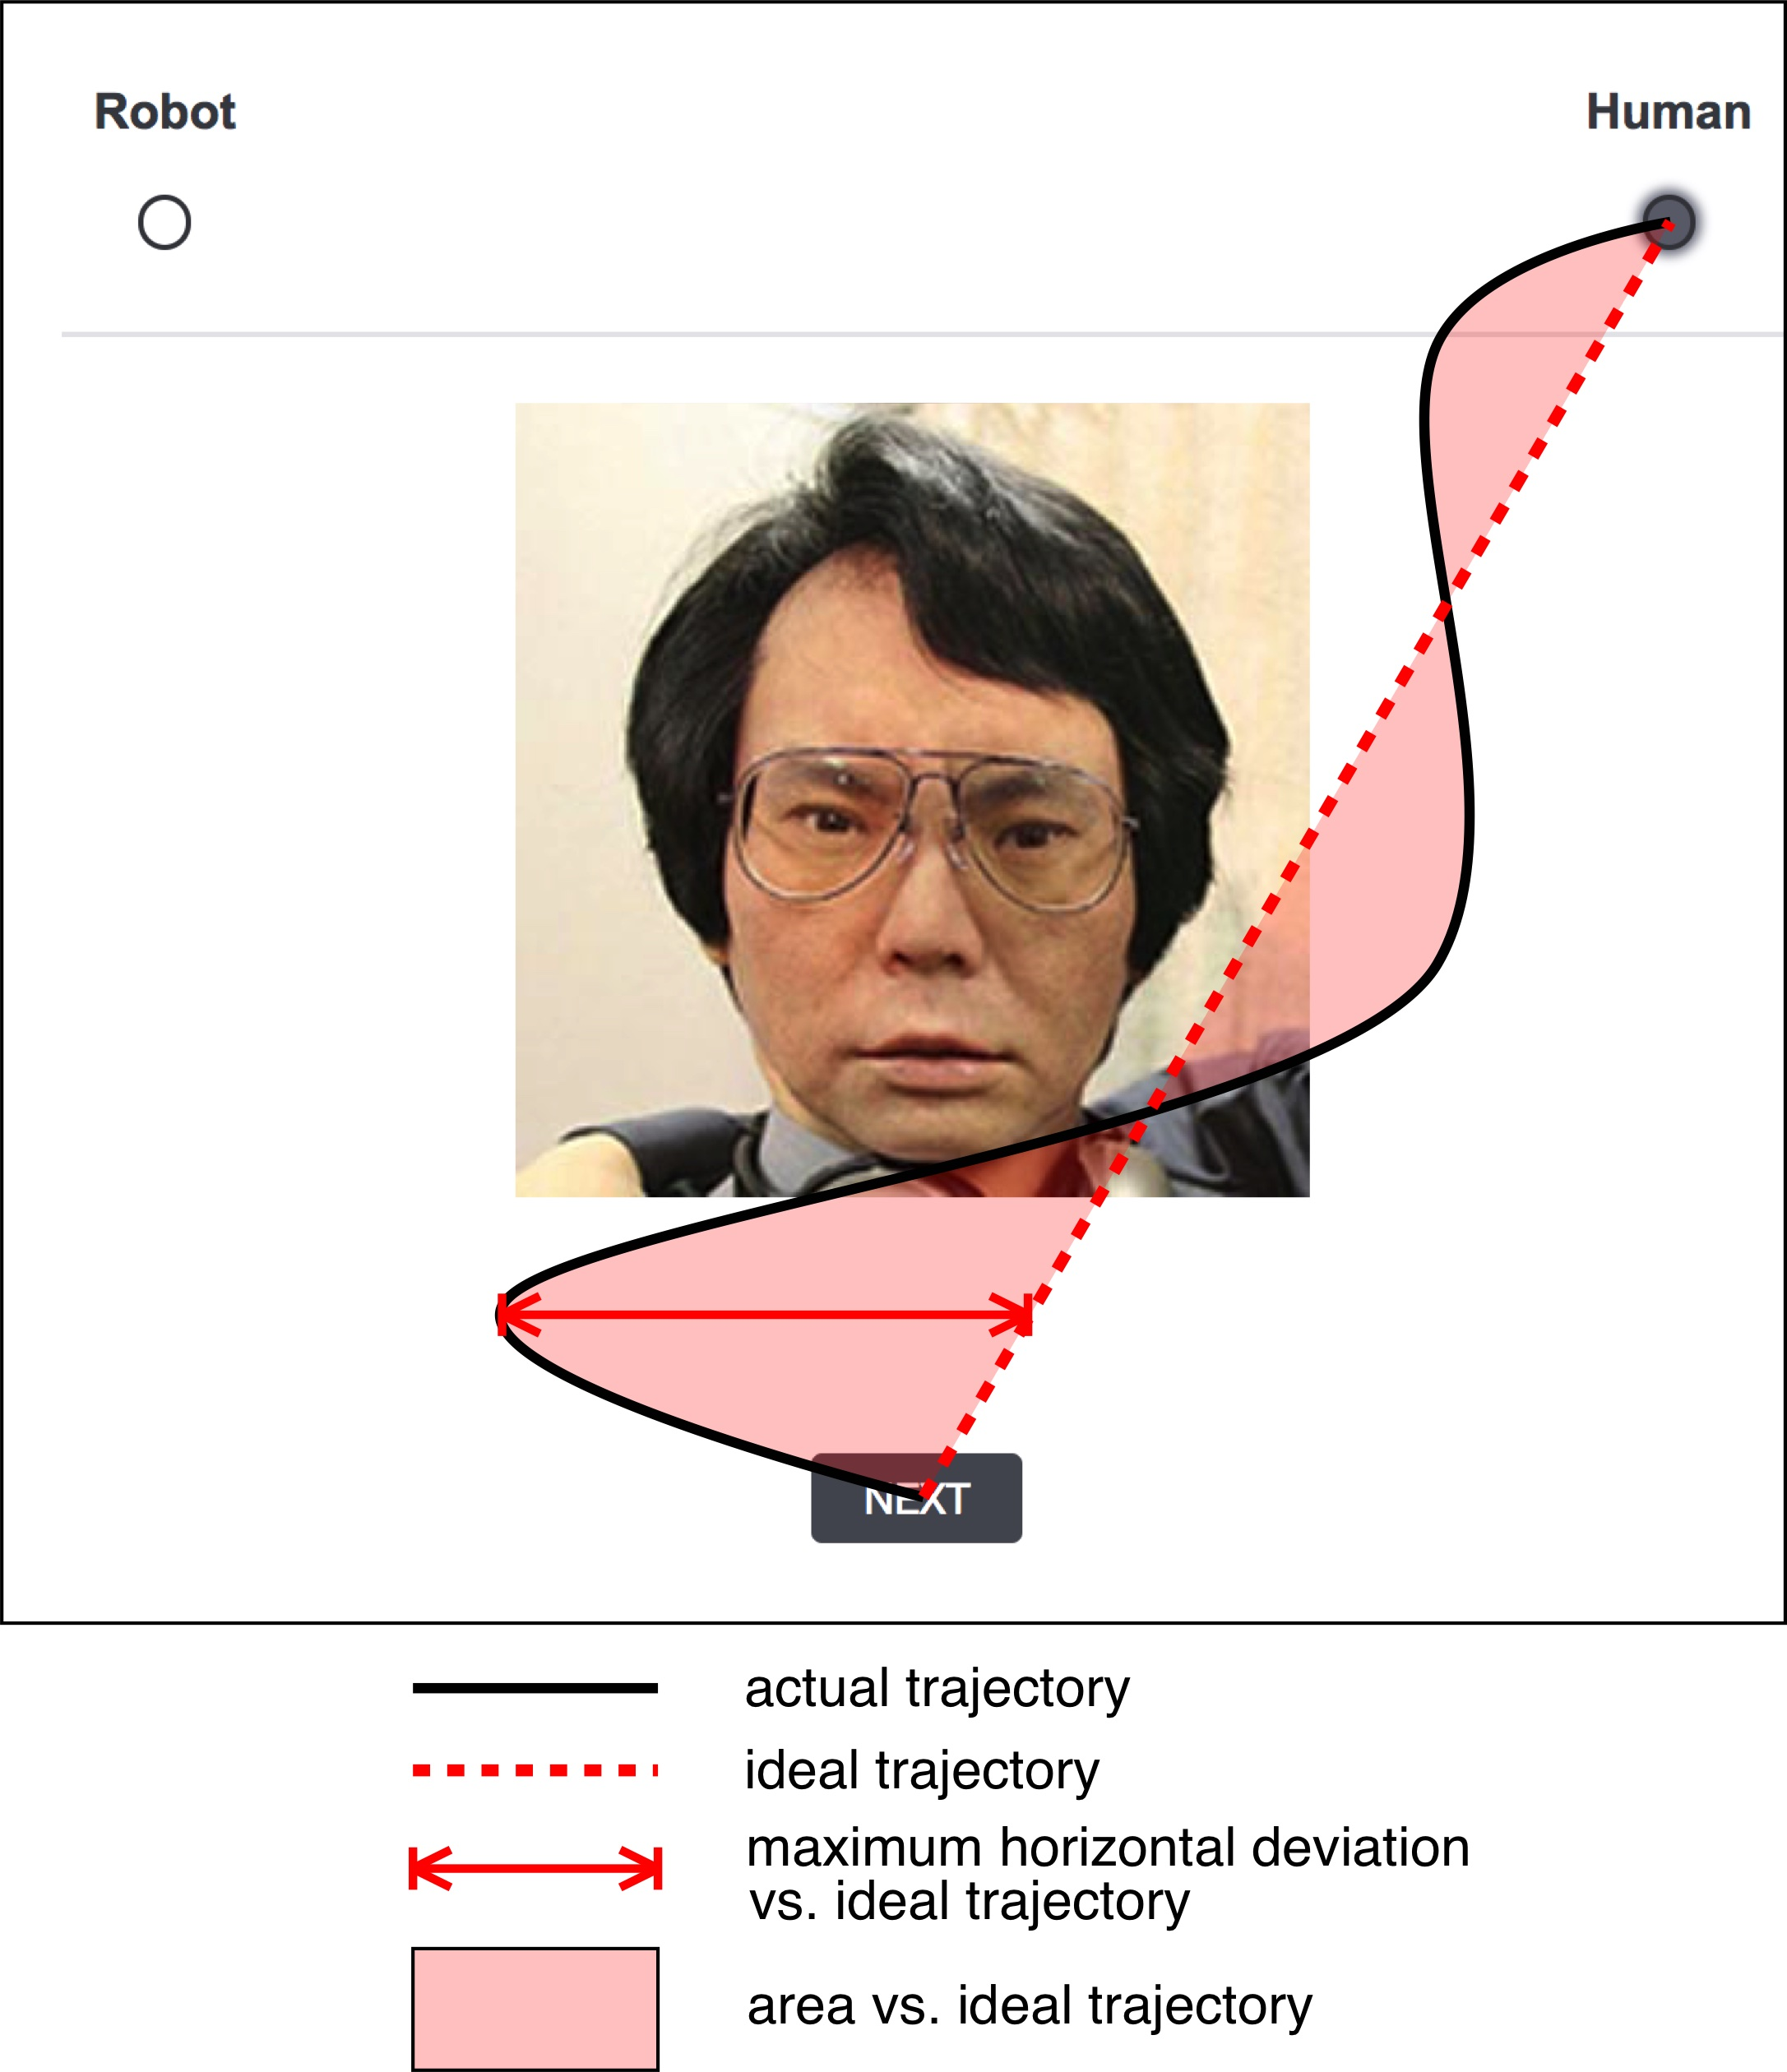
\includegraphics[width=110mm]{Figures/Figure 1.jpeg}
\caption{\label{fig:diagram}Typical outcome measures for category-competition experiments. In this example, a hypothetical subject's cursor trajectory suggests initial attraction to the "robot" category, but in an early change of direction, the subject appears to become more attracted to the "human" category. There is a final, weak attraction once again to the "robot" category, but the subject ultimately categorizes the face as "human". In our implementation, there is a 570-px horizontal distance between the category buttons and a 472-px vertical distance between the category buttons and the middle of the Next button.}
\end{figure}

Collecting reliable mouse trajectories that are comparable across
subjects and trials requires precise control over the visual layout and
timing of the experiment, as we will describe. Perhaps for this reason,
mouse-tracking experiments to date have usually been conducted in
person, with subjects physically present in the lab (with some
exceptions, e.g., Freeman et al. (2016)). Such settings allow for a
consistent visual presentation of the experiment through the use of
existing mouse-tracking software (Freeman \& Ambady, 2010; Kieslich \&
Henninger, 2017). In contrast, collecting mouse-tracking data online,
for example through crowd-sourcing websites, could allow for much larger
samples, greater demographic diversity (Gosling, Sandy, John, \& Potter,
2010), and the possibility of implementing the same experiment in
multiple collaborating labs without special hardware or software
requirements. We are not aware of existing open-source software that is
suitable for these settings, that can accommodate common experimental
features such as presentation of multiple stimuli and randomization, and
that ensures a consistent, validated experimental presentation even when
subjects complete the study from their home computers or other devices.

The present paper therefore provides open-source software enabling
reliable and precise design of mouse-tracking experiments through the
widely used software Qualtrics (Provo, UT, last accessed 10-2018), a
graphical user interface that is designed for online data collection
that interfaces easily with crowd-sourcing websites such as Amazon
Mechanical Turk. Our software pipeline consists of: (1) a premade
Qualtrics template containing embedded Javascript and CSS that manages
stimulus presentation, trains subjects on the experimental task, and
collects mouse trajectory and time data; and (2) R code to clean, parse,
and analyze the data. We present a validation study demonstrating
consistent data collection even in relatively uncontrolled online
settings and demonstrating that these methods show concurrent validity
when benchmarked using previously tested stimuli.

\section{A basic category-competition experiment}
\label{sec:basic_expt}

In a standard category-competition experiment, the subject views a
series of stimuli presented sequentially on separate pages. The subject
must categorize each stimulus by clicking on one of two buttons
presented on the left and right sides of the window (Figure
\ref{fig:diagram}). Stimuli are typically chosen such that some fall
clearly into one of the categories, while others are ambiguous or
difficult to categorize. Ambiguous stimuli are thought to activate
mental representation of both categories simultaneously, leading to
dynamic competition that manifests in real time as unstable mouse
dynamics (Freeman \& Johnson, 2016). That is, because the subject is
continuously or alternately attracted to both categories, the mouse
trajectory may contain frequent direction changes and may diverge
substantially from a direct path from the start position to the location
of the category button ultimately chosen.

Specifically, past literature (e.g., Freeman et al. (2008)) has used
several outcome measures to operationalize category competition through
mouse dynamics. More ambiguous stimuli typically increase the number of
times the subject's mouse changes directions horizontally
(\emph{$x$-flips}). Additionally, compared to unambiguous stimuli,
ambiguous stimuli tend to produce trajectories that diverge more from an
``ideal trajectory'' consisting of a straight line from the subject's
initial cursor position to the finally chosen radio button (Figure
\ref{fig:diagram}, red dashed line). That is, the
\emph{maximum horizontal deviation} between the ideal trajectory and the
subject's actual trajectory (Figure \ref{fig:diagram}, red solid line),
as well as the \emph{area} between the ideal and actual trajectories
(Figure \ref{fig:diagram}, pink shading), are typically larger for
ambiguous stimuli. Our implementation calculates these measures using
trajectories rescaled to unit length in both the \(x\)- and
\(y\)-dimensions and calculates the area using Riemann integration.
Other outcome measures can include the \emph{maximum speed} of the
subject's cursor (ambiguous stimuli tend to produce higher maximum
speeds, reflecting abrupt category shifts (Freeman et al., 2016)) and
the total reaction time for the trial (ambiguous stimuli tend to produce
longer reaction times). We calculate reaction time as the time elapsed
between the start of the trial, after the page is fully loaded, to the
time at which the subject clicks on a button to categorize the stimulus.
However, both maximum speed and reaction time have limitations and are
perhaps best treated as secondary measures (Freeman et al., 2016).

\section{How to create and analyze an experiment with our software}

Our open-source software provides a user-friendly data collection and
analysis pipeline for creating such experiments as follows. First, the
user imports into Qualtrics a template questionnaire
(\url{https://osf.io/st2ef/}) implementing the validation study
presented below. The key feature is two question ``blocks'' that present
the stimuli sequentially, in randomized order, via Qualtrics' ``Loop \&
Merge'' feature; other blocks in the survey, such as one presenting
demographic questions, can be added or removed as needed. The image URLs
in the Loop \& Merge can simply be edited through the Qualtrics
interface to replace the default stimuli. The first block of the
questionnaire shows instructions (Online Supplement). Then the first
Loop \& Merge block presents training stimuli to acclimitize the subject
to the experiment, including to alert messages designed to optimize
subject behavior for mouse-tracking, detailed in Section
\ref{sec:opt_behav} below. The second Loop \& Merge block of
experimental stimuli begins data collection by activating
mouse-tracking. The underlying Javascript that activates
mouse-tracking\footnote{The Javascript code is already embedded in the template Qualtrics files, but it is also available as standalone files (\url{https://osf.io/st2ef/}).}
requires no modification except that global variables specifying the
number of training stimuli (\texttt{howManyPracticeImages}, defaulting
to 6) and real experimental stimuli (\texttt{howManyRealImages},
defaulting to 10) must be changed to match the number of user-supplied
stimuli. Additional parameters that the user can optionally change are
listed in Table \ref{tb:js_parameters}. The Qualtrics template also
contains (in the ``Look and Feel'' section accessible through the
Qualtrics user interface) a small snippet of CSS that formats the radio
buttons.\footnote{The CSS code is also available as a standalone file (\url{https://osf.io/st2ef/}).}
The Qualtrics questionnaire is then ready to collect data.

\begin{table}[h]
\caption{Modifiable Javascript global variables}
\label{tb:js_parameters}
\centering
\begin{tabular}{@{}ccc@{}}
\toprule
\textbf{Variable}             & \textbf{Default}      & \textbf{Meaning}                                      \\ \midrule
%--
\texttt{howManyPracticeImages}         & 6    & The number of practice stimuli (for which no mouse trajectories will \\&&be recorded)                               \\ \\
%--
\texttt{howManyRealImages}               & 10 & The number of experimental stimuli (for which mouse trajectories will \\&&be recorded)                               \\ \\
%--
\texttt{maxAnswerTime}       & 5000    & The maximum time (ms) that can be spent on a trial. \\&&Trials with longer answer times will receive a "took too long" alert.                                                                   \\ \\
%--
\texttt{maxLatency}              & 700 & The maximum time (ms) after trial onset for which subject can \\&&leave mouse position unchanged. \\&&Trials with longer latencies will receive a "started too late" alert. \\
\bottomrule
\end{tabular}
\end{table}

After data collection, the raw Qualtrics dataset in wide format will
contain columns with continuous records of the subjects' mouse
coordinates (\texttt{xPos} and \texttt{yPos}), the absolute time (ms
since January 1, 1970, 00:00:00 UTC, which is the standard origin time
in Javascript) at which these coordinates were recorded (\texttt{t}),
the times at which each trial began (\texttt{onReadyTime}), and the
times at which the subject chose a category button
(\texttt{buttonClickTime}). These variables are recorded as a single
string for each subject with a special character ``a'' separating the
individual recordings, enabling easy parsing in R or another analysis
software. That is, \texttt{onReadyTime} and \texttt{buttonClickTime} are
sampled once per trial, while \texttt{xPos}, \texttt{yPos}, and
\texttt{t} are sampled as a triplet approximately every 16-18
ms\footnote{Specifically, our Javascript function for recording mouse
  position (\texttt{getMousePosition}) is triggered by ``mousemove''
  events issued by the browser. Therefore, the frequency of mousemove
  events determines the minimum time interval for measuring mouse
  position. The current World Wide Web Consortium standards (``UI
  events,'' 2018) do not specify a frequency at which browsers should
  issue mouse events, but at the time of writing, the most common
  browsers use a de facto standard 60-Hz rate (to match the most common
  display screen refresh rate). Other factors may also contribute to the
  sampling rate, including mouse DPI (how many positions are reported by
  the mouse per inch of movement), the system's USB polling rate (how
  often the mouse is queried for data), and potential variable lag due
  to high demand on CPU resources. However, in practice we have found
  that the effect of these factors must be minimal because our median
  mouse position interval (17 ms) agrees well with the 60-Hz event
  reporting interval of 16.7 ms.}. Additionally, the user's browser,
browser version, operating system, and browser resolution are recorded.
Table \ref{tb:wide_codebook} provides details on these variables, along
with additional variables that are collected in the raw Qualtrics data
but were not used in the present analyses.

The R code in \texttt{data\_prep.R} automatically checks the data for
idiosyncratic problems, returning a list of subjects flagged for
possible exclusion, along with reasons (see Section \ref{sec:special}
below for details). The R code then parses the raw data downloaded from
Qualtrics, computes the outcome measures described above, and returns
the dataset in an analysis-ready format. Specifically, the code first
parses the character-separated strings into a list for each subject,
each of which contains a list for each experimental stimulus. For
example, a particular subject might have the following \(x\)-coordinate
lists for the first three stimuli (prior to rescaling the trajectories
to unit length):

\begin{Shaded}
\begin{Highlighting}[]
\NormalTok{[[}\DecValTok{1}\NormalTok{]]}
\NormalTok{ [}\DecValTok{1}\NormalTok{] }\DecValTok{947} \DecValTok{946} \DecValTok{946} \DecValTok{946} \DecValTok{946} \DecValTok{944} \DecValTok{941} \DecValTok{938} \DecValTok{936} \DecValTok{934} \DecValTok{932} \DecValTok{927} \DecValTok{922} \DecValTok{916} \DecValTok{910}
\NormalTok{[}\DecValTok{16}\NormalTok{] }\DecValTok{908} \DecValTok{906} \DecValTok{903} \DecValTok{899} \DecValTok{894} \DecValTok{887} \DecValTok{880} \DecValTok{874} \DecValTok{867} \DecValTok{859} \DecValTok{850} \DecValTok{839} \DecValTok{829} \DecValTok{815} \DecValTok{803}
\NormalTok{[}\DecValTok{31}\NormalTok{] }\DecValTok{794} \DecValTok{786} \DecValTok{777} \DecValTok{768} \DecValTok{758} \DecValTok{750} \DecValTok{744} \DecValTok{736} \DecValTok{728} \DecValTok{723} \DecValTok{719} \DecValTok{717} \DecValTok{714} \DecValTok{709} \DecValTok{703}
\NormalTok{[}\DecValTok{46}\NormalTok{] }\DecValTok{700} \DecValTok{696} \DecValTok{692} \DecValTok{690} \DecValTok{689} \DecValTok{687} \DecValTok{684} \DecValTok{681} \DecValTok{680} \DecValTok{678} \DecValTok{676} \DecValTok{675} \DecValTok{674} \DecValTok{672} \DecValTok{670}
\NormalTok{[}\DecValTok{61}\NormalTok{] }\DecValTok{669} \DecValTok{668} \DecValTok{668}

\NormalTok{[[}\DecValTok{2}\NormalTok{]]}
\NormalTok{ [}\DecValTok{1}\NormalTok{] }\DecValTok{972} \DecValTok{968} \DecValTok{964} \DecValTok{960} \DecValTok{956} \DecValTok{951} \DecValTok{946} \DecValTok{939} \DecValTok{927} \DecValTok{917} \DecValTok{908} \DecValTok{900} \DecValTok{888} \DecValTok{876} \DecValTok{862}
\NormalTok{[}\DecValTok{16}\NormalTok{] }\DecValTok{847} \DecValTok{831} \DecValTok{816} \DecValTok{801} \DecValTok{784} \DecValTok{772} \DecValTok{763} \DecValTok{753} \DecValTok{743} \DecValTok{733} \DecValTok{725} \DecValTok{721} \DecValTok{715} \DecValTok{709} \DecValTok{704}
\NormalTok{[}\DecValTok{31}\NormalTok{] }\DecValTok{699} \DecValTok{696} \DecValTok{694} \DecValTok{692} \DecValTok{689} \DecValTok{685} \DecValTok{683} \DecValTok{682} \DecValTok{679} \DecValTok{676} \DecValTok{675} \DecValTok{674} \DecValTok{674} \DecValTok{673} \DecValTok{672}
\NormalTok{[}\DecValTok{46}\NormalTok{] }\DecValTok{671} \DecValTok{671}

\NormalTok{[[}\DecValTok{3}\NormalTok{]]}
\NormalTok{ [}\DecValTok{1}\NormalTok{] }\DecValTok{988} \DecValTok{987} \DecValTok{986} \DecValTok{982} \DecValTok{977} \DecValTok{972} \DecValTok{966} \DecValTok{961} \DecValTok{953} \DecValTok{942} \DecValTok{927} \DecValTok{910} \DecValTok{894} \DecValTok{878} \DecValTok{866}
\NormalTok{[}\DecValTok{16}\NormalTok{] }\DecValTok{849} \DecValTok{826} \DecValTok{808} \DecValTok{792} \DecValTok{781} \DecValTok{771} \DecValTok{761} \DecValTok{751} \DecValTok{745} \DecValTok{741} \DecValTok{738} \DecValTok{733} \DecValTok{729} \DecValTok{725} \DecValTok{722}
\NormalTok{[}\DecValTok{31}\NormalTok{] }\DecValTok{719} \DecValTok{715} \DecValTok{710} \DecValTok{707} \DecValTok{704} \DecValTok{701} \DecValTok{699} \DecValTok{696} \DecValTok{693} \DecValTok{689} \DecValTok{686} \DecValTok{685} \DecValTok{683} \DecValTok{682} \DecValTok{681}
\NormalTok{[}\DecValTok{46}\NormalTok{] }\DecValTok{679} \DecValTok{678} \DecValTok{676} \DecValTok{676} \DecValTok{676}
\end{Highlighting}
\end{Shaded}

In the process, the code accounts for the possibility of
order-randomized Loop \& Merge iterates by appropriately reordering the
coordinate and time data. The outcome measures are computed for each
subject and appended to the wide-format dataset. By default, our
analysis code defines the time variable as the time elapsed from the
beginning of each trial, specifically the time at which the page was
loaded. Note that if the trajectories are to be directly averaged rather
than used to compute the outcome measures we describe, the times should
be standardized to account for differences in the times elapsed for each
trial (Freeman \& Ambady, 2010). This can be accomplished simply by
passing the argument \texttt{rescale\ =\ TRUE} to the function
\texttt{get\_subject\_lists} when parsing the time data. Additional
outcome measures, such as trajectory curvature (Dale et al., 2007;
Kieslich \& Hilbig, 2014; Wojnowicz et al., 2009) or speed profiles
throughout a trial (Freeman et al., 2016), could also be easily
calculated from the raw coordinate data supplied by the provided R
scripts. Finally, the dataset is reshaped into an analysis-friendly long
format, such that there is one row for each trial rather than for each
subject:

\begin{Shaded}
\begin{Highlighting}[]
\NormalTok{  id   cat xflips  xdev   area   speed rxnt }
\DecValTok{1}  \DecValTok{1}\NormalTok{ Robot      }\DecValTok{0} \FloatTok{0.132} \FloatTok{0.0599} \FloatTok{0.00295} \DecValTok{1048}         
\DecValTok{2}  \DecValTok{2}\NormalTok{ Robot      }\DecValTok{0} \FloatTok{0.112} \FloatTok{0.0577} \FloatTok{0.00906}  \DecValTok{701}         
\DecValTok{3}  \DecValTok{3}\NormalTok{ Robot      }\DecValTok{1} \FloatTok{0.225} \FloatTok{0.1638} \FloatTok{0.00776} \DecValTok{1184}         
\DecValTok{4}  \DecValTok{4}\NormalTok{ Robot      }\DecValTok{2} \FloatTok{0.266} \FloatTok{0.1473} \FloatTok{0.00328} \DecValTok{2022}         
\DecValTok{5}  \DecValTok{5}\NormalTok{ Robot      }\DecValTok{2} \FloatTok{0.254} \FloatTok{0.1129} \FloatTok{0.00655} \DecValTok{1410}         
\DecValTok{6}  \DecValTok{6}\NormalTok{ Robot      }\DecValTok{2} \FloatTok{0.254} \FloatTok{0.1180} \FloatTok{0.01493} \DecValTok{1037}         
\end{Highlighting}
\end{Shaded}

(Note that the outcome measures \texttt{xflips}, \texttt{xdev}, and
\texttt{area} are computed using rescaled trajectories, so are
unitless.) The code also prints information about alert messages
displayed to subjects, discussed in the next section. Although analysis
methods will differ by substantive application, we provide an example R
file, \texttt{analysis.R}, which conducts the analyses described in
Section \ref{sec:validation} below.

\singlespacing

\begin{table}[H]
\caption{Codebook of mouse-tracking, timing, and computing system variables in raw Qualtrics data}
\label{tb:wide_codebook}
\centering
\begin{tabular}{@{}ccc@{}}
\toprule
\textbf{Variable}             & \textbf{Units}      & \textbf{Meaning}                                      \\ \midrule
%--
\texttt{xPos}              & px & $x$-coordinate of cursor relative to upper left-hand \\&&corner of browser window \\ \\
%--
\texttt{yPos}              & px & $y$-coordinate of cursor relative to upper left-hand corner \\ \\
%--
\texttt{time}              & \makecell{ms since 1970-01-01 \\0:00:00 UTC} & Time at which each coordinate pair was measured  \\ \\
%--
\texttt{onLoadTime}         & \makecell{ms since 1970-01-01 \\0:00:00 UTC}    &  Time at which page for each trial started loading                         \\ \\
%--
\texttt{onReadyTime}               & \makecell{ms since 1970-01-01 \\0:00:00 UTC} & Time at which the page for each trial was loaded \\&&(beginning of trial)                              \\ \\
%--
\texttt{buttonClickTime}       & \makecell{ms since 1970-01-01 \\0:00:00 UTC}    & Time at which subject made category decision \\&&(end of trial)                                                                   \\ \\
%--
\texttt{pageSubmitTime}              & \makecell{ms since 1970-01-01 \\0:00:00 UTC} & Time at which subject proceeded to next trial by \\&&clicking "Next" \\ \\
%--
\texttt{windowWidth}              & px & Width of subject's browser window at beginning of trial\\ \\
%--
\texttt{windowHeight}              & px & Height of subject's browser window at beginning of trial \\ \\
%--
\texttt{alerts}              & N/A & Alerts received during each trial: \\&&0 = none \\&&1 = started too early \\&&2 = started too late \\&&3 = surpassed time limit for trial \\&&4 = window too small to fully display experiment \\ \\
%--
\texttt{latency}              & ms & Time between \texttt{onReadyTime} and first mouse move \\ \\
%--
\texttt{stimulusOrder}              & N/A & Stimulus URLs for each trial in the order presented to \\&&subject \\ \\
%--
\texttt{browser\_Browser}              & N/A & Internet browser \\ \\
%--
\texttt{browser\_Version}              & N/A & Browser version\\ \\
%--
\texttt{browser\_Operating.System}              & N/A & Operating system \\ \\
%--
\texttt{browser\_Resolution}              & N/A & Browser resolution \\
\bottomrule
\end{tabular}
\end{table}

\singlespacing

\section{Methodological details}

\subsection{Optimizing subject behavior for mouse-tracking}
\label{sec:opt_behav}

If subjects sometimes make their category decisions prior to moving
their mouse cursors -- that is, if they wait to begin moving their
cursors until they have already made a decision -- then their mouse
trajectories may begin too late to capture dynamic category competition
(Freeman et al., 2016). For this reason, at the end of each trial in
which the subject took more than 700 ms (by default) to begin moving the
cursor, the questionnaire issues a ``started too late'' alert warning
the subject to begin moving the cursor faster at the beginning of each
trial. Additionally, to encourage fast decision-making and discourage
subjects from taking unscheduled breaks from the experiment, after any
trial in which the subject takes longer than 5000 ms (by default) to
make a category decision, the questionnaire issues a ``took too long''
alert reminding the subject to answer more quickly (Freeman et al.,
2016). Some investigators choose not to limit total response time (e.g.,
Kieslich \& Hilbig (2014)), in which case the parameter
\emph{maxLatencyTime} could simply be set to a very large value, such as
50,000 ms. All alerts are recorded in the dataset at the time they are
triggered, but to avoid disrupting the subject's behavior during the
trial, they are not displayed onscreen until after the subject selects a
category button, but before the subject clicks the Next button to
proceed to the next trial. The recorded alert data allow investigators
to exclude trials or subjects receiving certain types of alerts if
desired. The full text of all alert messages appears in the Online
Supplement.

\subsection{Special considerations for online use}

\label{sec:special}

As mentioned, allowing subjects to complete the experiment on their own
devices, rather than in a controlled lab setting, poses several
challenges to collecting reliable and precise mouse-tracking data. For
example, the software cannot precisely position the subject's cursor at
the start of each trial; browsers do not provide this functionality to
preclude malicious misuse. Furthermore, the experiment interface is
displayed with the same pixel dimensions for every subject and trial,
regardless of the size and resolution of each subject's screen,
potentially yielding interfaces of somewhat differing visual sizes for
different subjects. Fixing the visual size, rather than the pixel
dimensions, of the experiment interface across subjects was not feasible
because the survey software does not have reliable access to data on
each subject's screen size and resolution. Additionally, if subjects
attempted to complete the experiment with a browser window that is
smaller than the size of the the experiment interface (for example,
because their devices' screens are physically too small), then they
might have to scroll in the middle of each trial, leading to
non-continuous mouse trajectories and erroneous reaction times.

Our Javascript implementation addresses each of these possibilities. To
ensure that the cursor starts in an approximately fixed location, the
Next button, which is the necessary ending point for the cursor on every
trial, is positioned in the same location on every trial. Furthermore,
if the subject moves the cursor away from this position before the next
trial begins (i.e., while the page is loading), the questionnaire issues
a ``started too early'' alert warning the subject not to begin moving
the cursor before the page is loaded. During the first training trial,
the code checks the pixel dimensions of the subject's browser window,
and if the window is smaller than the expected pixel dimensions of the
experiment interface, the questionnaire issues an alert instructing the
subject to increase the window size until the stimulus image, both radio
buttons, and the submit button are fully visible. On subsequent trials,
the subject's ability to scroll is disabled, such that subjects using
devices with too-small screens or browser windows will not have access
to the Next button and will thus be unable to proceed through the
experiment.

As mentioned above, the use of fixed pixel dimensions does not guarantee
that the visual distance between the buttons will be the same for every
subject due to the many possible combinations of different physical
dimensions of computer monitors and different pixel-per-inch
resolutions. In addition, some subjects might use their browser's zoom
function, changing both the pixel distances and the visual distances.
Therefore, our R analysis code by default rescales all trajectories to
unit length in both the \(x\)- and \(y\)-dimensions. However, the
validation study described in Section \ref{sec:validation} below found
systematically larger values of the outcome measures for subjects with
trajectories suggesting non-standard pixel scaling due, for example, to
zooming typically showed larger values of the outcome measures. These
differences persisted despite that the trajectories had been rescaled to
unit length. Importantly, despite these mean differences on the outcome
measures, the key stimulus ambiguity effects were comparable between
subjects with non-standard pixel scaling and subjects with standard
pixel scaling. In practice, then, investigators might choose to simply
adjust analysis models for covariates indicating whether a subject had
non-standard pixel scaling (operationalized as having unexpectedly large
or small pixel distances between the starting and ending
\(x\)-coordinates on any trial) and whether a subject had ever had a
too-small window; this is the approach we adopt in the validation study.
Because the experimental manipulation is randomized, these
idiosyncrasies of the visual display size effectively introduce
``non-differential'' noise in the continuous outcome measures, in which
case the estimate for the effect of stimulus ambiguity remains unbiased
even without adjustment for the scaling and window size variables
(Rothman, Greenland, Lash, \& others, 2008). Thus, estimates should be
comparable across samples with different frequencies of non-standard
scaling and too-small windows. However, adjusting for these variables as
``precision covariates'' may improve statistical power by removing some
of the residual variation on the outcome measures that is due to these
visual idiosyncrasies rather than to stimulus ambiguity. The provided R
code automatically includes these two indicator variables (called
\texttt{weird.scaling} and \texttt{wts}, respectively) in the prepared
long-format dataset. Alternatively, subjects displaying these
idiosyncrasies could simply be excluded.

As an additional data quality concern in online settings, it is
sometimes possible for automated ``bots'' to complete Mechanical Turk
tasks, yielding invalid data (Difallah, Demartini, \& Cudré-Mauroux,
2012). Because bots do not physically use computer mice or trackpads to
proceed through the questionnaire, but rather select buttons directly,
they would not provide any mouse trajectories at all for our data
collection system to erroneously record. If a bot managed to complete
the questionnaire and respond to any alerts in the process, our data
preparation script would automatically flag its data for exclusion due
to missing trajectories.

\subsection{Extensions to other survey platforms}

This software is tailored to the Qualtrics survey platform. However,
because the specialized functions that manage the collection of mouse
trajectory and timing data are entirely contained in the Javascript,
this code could be readily adapted to other online survey platforms or
custom experimental interfaces as long as they are able to: (1) support
addition of custom Javascript, and provide a Javascript API with basic
functions similar to Qualtrics' \texttt{addOnReady}, \texttt{addOnLoad},
\texttt{disableNextButton}, \texttt{enableNextButton}, and
\texttt{setEmbeddedData}; (2) present multiple stimuli iteratively,
while recording their possibly randomized order; and (3) display the
experiment at fixed pixel dimensions. In short, to use this software on
another platform, an investigator would need to use that platform's user
interface to adjust the questionnaire display and flow to imitate our
Qualtrics-implemented design and would need to add our custom
Javascript, replacing the small number of calls to the Qualtrics API
with the relevant functions for the investigator's own platform.
Additionally, the values of some Javascript global variables related to
the display of the experiment, such as \texttt{minWindowWidth} and
\texttt{minWindowHeight}, might require modification. The Javascript is
thoroughly commented to facilitate such adaptation and further
modification by other users. Finally, it would also be possible for
investigators with experience coding in HTML to create a simple survey
platform, incorporating our Javacsript code, that could be hosted on
their own servers or used to run subjects in the lab.

\subsection{Limitations}

Our implementation has limitations. Occasional idiosyncrasies (e.g.,
extremely poor quality connections, use of proxy servers) can cause
losses of coordinate data for some trials or subjects. Our R code
automatically checks for subjects with these data losses and creates a
list of subject IDs that should be excluded, along with reasons for
exclusion. The validation study presented below suggested that these
issues affect a small fraction of trials for approximately 10\% of
subjects when data are collected in an uncontrolled crowdsourcing
setting. A conservative analysis approach, which we adopt in the
validation study, could be to exclude every subject with data losses on
any trial.

Additionally, our implementation cannot control subjects' individual
mouse speed settings. That is, different mice and trackpads may be set
to respond with larger or smaller onscreen movements for any given
physical movement of the subject's hand, and these differences in mouse
dynamics could affect the confusion measures. Because our implementation
collects data through an Internet browser, it is not able to measure
subjects' mouse speeds independently of, for example, their hand speeds.
However, like the visual idiosyncrasies produced by non-standard pixel
scaling or small browser windows, we would expect differences in mouse
speed settings to introduce only non-differential noise in the outcomes
and thus not compromise estimation of stimulus ambiguity effects (albeit
with some loss of statistical power).

Last, although our implementation appears to perform reliably across
common browsers (see Section \ref{sec:valid_results}), it is
incompatible with Internet Explorer; subjects running Internet Explorer
will be unable to proceed through the questionnaire, and no data will be
collected. (At present, Internet Explorer has only a 3\% share of
browser usage worldwide (``Browser market share worldwide,'' 2018).)
Finally, subjects with very slow Internet connections, causing image
stimuli to load slowly, may receive a large number of ``started too
late'' alerts, although their data will otherwise be useable. In
practice, subjects with a high frequency of ``started too late'' alerts
could be discarded if this were of concern.

\section{Validation study}
\label{sec:validation}

\subsection{Design and subjects}

To validate the provided software, we used it to perform a simple
category confusion experiment using image stimuli depicting the faces of
humanoid robots ranging from very mechanical to very humanlike. Previous
work (e.g., Mathur \& Reichling (2016), Mathur \& Reichling (2009))
suggests that humanoid robot faces that closely, but imperfectly,
resemble humans -- those occupying the ``Uncanny Valley'' (Mori, 1970)
-- can provoke intense feelings of eeriness, dislike, and distrust in
human viewers. One mechanism of these negative reactions may be that
robots occupying the Uncanny Valley provoke category confusion, which
may itself be aversive (Yamada, Kawabe, \& Ihaya, 2013). In partial
support for this hypothesis, Mathur \& Reichling (2016) found that robot
faces in the Uncanny Valley elicited the most category confusion. As a
validation, we attempted to conceptually reproduce Mathur \& Reichling
(2016)'s findings using the mouse-tracking software presented here. From
Mathur \& Reichling (2016)'s stimuli, we arbitrarily selected five
``unambiguous'' faces not occupying the Uncanny Valley (Figure
\ref{fig:traj}, row 1) and five ``ambiguous'' faces occupying the
Uncanny Valley (Figure \ref{fig:traj}, row 2). Given previous findings
regarding these faces (Mathur \& Reichling, 2016), we expected mouse
trajectories to indicate greater average confusion for ambiguous faces
vs.~unambiguous faces. We analyzed mouse trajectories from \(n =\) 188
United States subjects recruited on Amazon Mechanical Turk from among
users with a prior task approval rating of at least 95\%. We compensated
subjects \$0.25 to complete the study and set a time limit of 20 minutes
for the entire task to discourage subjects from taking long breaks from
the study. Subjects used the template Qualtrics questionnaire provided
here to categorize each face as either a ``robot'' or a ``human''. We
randomized the order of stimulus presentation for each subject. A link
to a live demonstration version of the questionnaire is provided at
\url{https://osf.io/st2ef/}.

\subsection{Statistical analysis}

We regressed each of the five outcome measures described in Section
\ref{sec:basic_expt} on a binary indicator for stimulus ambiguity. For
ease of interpretation, we first standardized the four continuous
outcome variables (area, maximum x-deviation, peak speed, and reaction
time); thus, their coefficients represent the average number of standard
deviations by which the outcome measure was larger for ambiguous versus
unambiguous trials. Regression models were semiparametric generalized
estimating equations (GEE) models with a working exchangeable
correlation structure and robust inference, and the unit of analysis was
trials (1880 observations). We chose this specification in order to
account for arbitrary correlation structures within subjects and within
stimuli, as well as to avoid making distributional assumptions on the
residuals for highly-skewed outcomes such as reaction time. Models for
continuous outcomes used the identity link, while the model for
\(x\)-flips used the Poisson link. To account for residual variation in
the visual display size of the experiment as described in Section
\ref{sec:special} above, each outcome model included main effects of
indicator variables for non-standard pixel dimensions and for too-small
browser windows (the variables \texttt{weird.scaling} and \texttt{wts}),
as well as all possible interactions among these nuisance variables and
the stimulus ambiguity indicator. As a sensitivity analysis, we also
performed the analyses excluding all such subjects (for an analyzed
\(n=103\)) rather than adjusting for the nuisance covariates, yielding
nearly identical point estimates and inference.

\subsection{Results}

\subsubsection{Descriptive measures}

Table \ref{tb:subject_characteristics} displays demographic
characteristics of the analyzed subjects, as well as their Internet
browsers and operating systems. We collected data on 203 subjects (using
an \emph{a priori} sample size determination of \(n=200\)) and excluded
24 due to idiosyncratic timing issues, yielding an analyzed sample size
of 188. These exclusion criteria are conservative in that we excluded
all trials for any subject with these problems on any trial, even if
only a small number of trials were affected. As discussed in Section
\ref{sec:special}, our questionnaire also collects data on scaling and
window size idiosyncrasies that do still allow for normal data
collection but could in principle affect the confusion measures; of the
analyzed subjects, 18 had a too-small window on at least one trial, and
77 had non-standard pixel dimensions on at least one trial. No subject's
data indicated a clear violation of the instructions, so we compensated
all subjects who completed the study on Amazon Mechanical Turk.

Across all trials, subjects used a median browser window height of 775
px (\(25^{th}\) percentile: 726 px; \(75^{th}\) percentile: 938 px) and
a median window width of 1532 px (\(25^{th}\) percentile: 1366 px;
\(75^{th}\) percentile: 1846 px). Across all trials, the median reaction
time was 1170 ms (\(25^{th}\) percentile: 859 ms; \(75^{th}\)
percentile: 1628 ms). The average latency (that is, the time elapsed
between the beginning of the trial and the subject's first mouse
movement) was 442 ms (\(25^{th}\) percentile: 87 ms; \(75^{th}\)
percentile: 640 ms), which is short enough to suggest that the mouse
trajectories would have captured dynamic competition processes occurring
almost immediately after stimulus presentation. Across all sampled mouse
coordinate pairs, the median sampling rate was 17 times per second
(\(25^{th}\) percentile: 16 ms; \(75^{th}\) percentile: 18 ms). To
provide some reference for the frequency of alert messages that can be
expected, 68\% of trials received no alerts, and the remaining 32\% of
trials received a median of 1 alert (of a maximum of
4)\footnote{It may appear counterintuitive that a trial could receive all four alerts, including both "Started too early" and "Started too late". However, this can occur if the subject moves the cursor outside the Next button before the subsequent trial has fully loaded ("Started too early") but then, once the subsequent trial is loaded, waits too long to move the cursor again ("Started too late"). To avoid confusing the subject, in this situation, only the "Started too early" alert is displayed.}.
Table \ref{tb:alerts_trial} displays the relative frequencies of each
alert type among all alerts received, and Table \ref{tb:alerts_subject}
displays the percent of subjects receiving each alert type at least
once. The fairly high frequency of alerts is to be expected: as
discussed in Section \ref{sec:opt_behav}, the alerts, particularly those
instructing the subject to begin moving the cursor sooner or to avoid
moving it before the trial is fully loaded, are designed to optimize
subject behavior rather than to indicate invalid data.

\begin{table}[H]
\centering
\caption{\label{tb:subject_characteristics}Demographics and computing system characteristics for subjects in validation study.}
\begin{tabular}{@{}ll@{}}
\toprule
                                                          & Overall       \\ \midrule
Total N                                                   & 188           \\
Age (mean (SD))                                           & 36.80 (11.73) \\
Education (n (\%))                                             &               \\
\hspace{6mm}Did not graduate high school & 2 (1.1)       \\
\hspace{6mm}Graduated 2-year college     & 35 (18.6)     \\
\hspace{6mm}Graduated 4-year college     & 75 (39.9)     \\
\hspace{6mm}Graduated high school        & 54 (28.7)     \\
\hspace{6mm}Post-graduate degree         & 22 (11.7)     \\
Female (mean (sd))                                        & 0.52 (0.50)   \\
Race (n (\%))                                             &               \\
\hspace{6mm}Black/African American                        & 16 (8.5)      \\
\hspace{6mm}Caucasian                                    & 144 (76.6)    \\
\hspace{6mm}Native American                              & 8 (4.3)       \\
\hspace{6mm}East Asian                                    & 12 (6.4)      \\
\hspace{6mm}Hispanic                                      & 14 (7.4)      \\
\hspace{6mm}Middle Eastern                                & 4 (2.1)       \\
\hspace{6mm}Southeast Asian                               & 3 (1.6)       \\
\hspace{6mm}South Asian                                   & 2 (1.1)       \\ 
Browser (n (\%))                                               &               \\
\hspace{6mm}Chrome                       & 153 (81.4)    \\
\hspace{6mm}Edge                         & 2 (1.1)       \\
\hspace{6mm}Firefox                      & 33 (17.6)     \\ 
Operating system (n (\%))                                              &               \\
\hspace{6mm}Chrome OS                      & 7 (3.7)    \\
\hspace{6mm}Linux                         & 6 (3.2)        \\
\hspace{6mm}Macintosh                      & 19 (10.1)     \\
\hspace{6mm}Windows                      & 155 (82.4)     \\ \bottomrule
\end{tabular}
\end{table}

\begin{table}[H]
\centering
\caption{\label{tb:alerts_trial}Summary of all 711 alert messages received in validation study across all 1880 trials.}
\begin{tabular}{cc}
  \hline
 Alert type & \% of all alerts received\\ 
  \hline
Started too early & 40 \\ 
  Started too late & 31 \\ 
  Surpassed trial time limit & 8 \\ 
  Window too small & 21 \\ 
   \hline
\end{tabular}
\end{table}

\begin{table}[H]
\centering
\caption{\label{tb:alerts_subject}Percent of subjects (n=188) receiving each type of alert message at least once across 10 trials.}
\begin{tabular}{cc}
  \hline
Alert type & \% of subjects \\ 
  \hline
Started too early & 60 \\ 
  Started too late & 58 \\ 
  Surpassed trial time limit & 20 \\ 
  Window too small & 10 \\ 
   \hline
\end{tabular}
\end{table}

\subsubsection{Effect of stimulus ambiguity on mouse trajectories} 
\label{sec:valid_results}

As a visual example of the mouse trajectories, Figure \ref{fig:traj}
shows unit-scaled trajectories from the fifth subject. For this subject,
ambiguous faces 6, 8, and 9 in particular elicited mouse trajectories
characteristic of substantial category confusion, evidenced by
\(x\)-flips and large deviations from the ideal trajectory. (The reason
for the rightward trajectory for face 7 is that the subject classified
this face as ``Human'', whereas all the other faces were classified as
``Robot''.) Figure \ref{fig:violin} aggregates outcome data across
subjects in violin plots that display the medians of each standardized
outcome measure for ambiguous versus unambiguous stimuli, as well as
density estimates of their distributions. These results indicate
visually that each measure of confusion was on average higher for
ambiguous versus unambiguous stimuli. That is, aligning with the
predicted results discussed in Section \ref{sec:basic_expt}, subjects'
cursors appeared to make more horizontal changes of direction, to make
less direct paths, and to reach higher peak speeds for ambiguous versus
unambiguous stimuli, and furthermore trials for ambiguous stimuli
elicited longer reaction times. Point estimates from the GEE models of
the mean difference for each confusion measure for ambiguous versus
unambiguous stimuli (Figure \ref{fig:violin}) were in the predicted
direction for all stimuli (with \(p < 0.0001\) for all outcomes).
Collectively, these results suggest that the software and methods
presented here adequately capture confusion when implemented through
realistic crowdsourced data collection.

\begin{figure}[H]
\centering
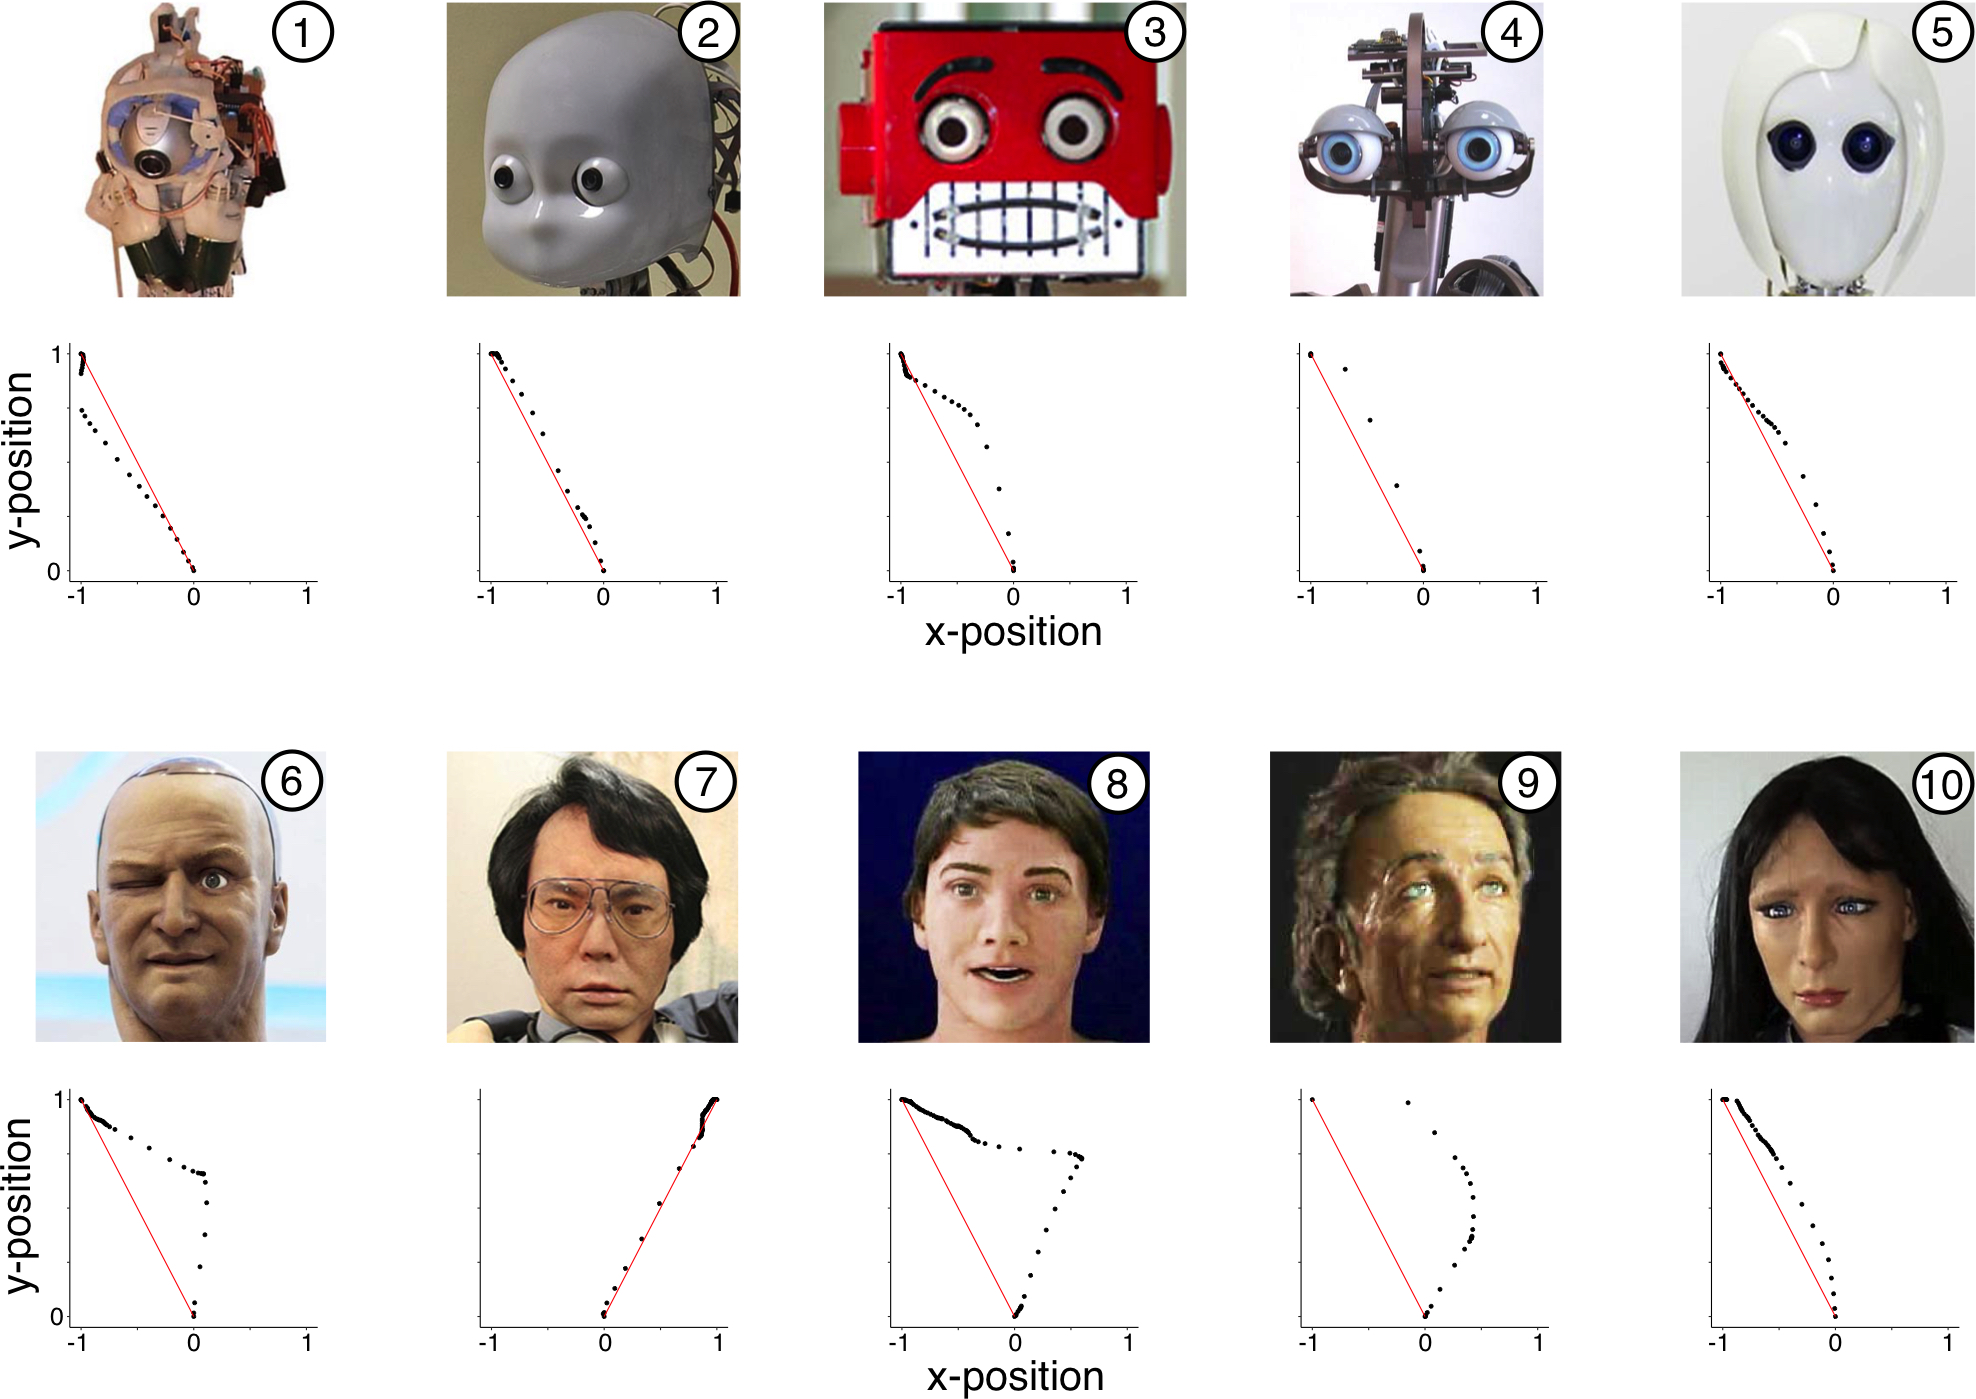
\includegraphics[width=150mm]{figures/Figure 2.jpeg}
\caption{\label{fig:traj}Mouse trajectories for a single subject categorizing unambiguous (top row) versus ambiguous (bottom row) humanoid robot faces. Trajectories have been rescaled to unit length in both the $x$- and $y$-dimensions.}
\end{figure}

\begin{figure}[H]
\centering
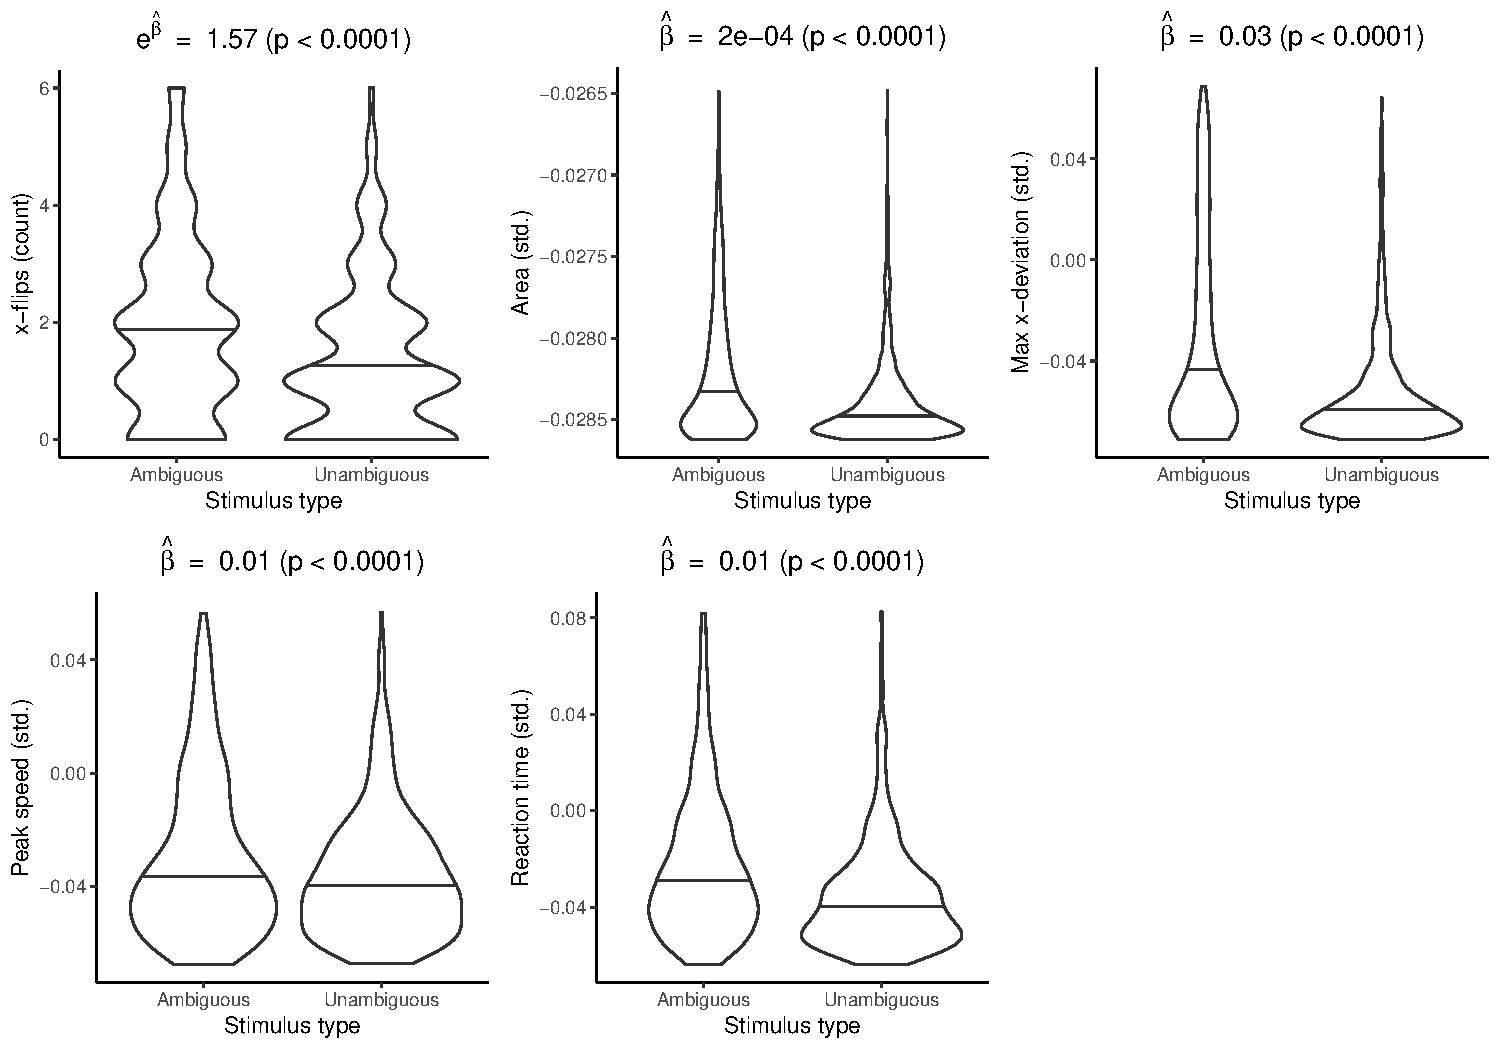
\includegraphics[width=150mm]{figures/violin_plots.pdf}
\caption{\label{fig:violin}Violin plots showing standardized outcome data for 1880 trials (188 subjects) for ambiguous versus unambiguous face stimuli. Violin contours are mirrored kernel density estimates. Horizontal lines within violins are medians. $\widehat{\beta}$ = GEE estimate of mean difference (ambiguous - unambiguous); $p$ = $p$-value for difference estimated by robust GEE inference.}
\end{figure}

\subsubsection{Consistency of results across computing systems}

As a post hoc secondary analysis to assess the consistency of these
stimulus ambiguity effects across browsers and operating systems, we
refit the regression models including interaction terms of browser
(Firefox vs.~Chrome) and of operating system (Macintosh vs.~Windows)
with stimulus ambiguity. The resulting coefficients thus estimate the
differences in the stimulus ambiguity effect on confusion between
browsers or between operating systems. We excluded subjects who used
other, much less common, browsers and operating systems due to their
small sample sizes, yielding 1720 trials in this analysis. Across the
five outcome models, the browser interaction coefficients ranged in
absolute value from 0.03 to 0.28 with \(p\)-values from 0.32 to 0.54,
and the operating system interaction coefficients ranged in absolute
value from 0.004 to 0.26 with \(p\)-values from 0.14 to 0.62. While this
validation study was not specifically powered to assess for differences
in results across browsers and operating system effects, these results
suggest that any such effects are likely fairly small.

\section{Reproducibility}

All data, code, and materials required to reproduce the validation study
are publicly available and documented (\url{https://osf.io/st2ef/}).

\section{Online supplement}

The Online Supplement, containing the instructions and alert messages
displayed to subjects, is publicly available
(\url{https://osf.io/83jze/}).

\section{Acknowledgments}

This research was supported by NIH grant R01 CA222147 and by a Harvard
University Mind, Brain, \& Behavior grant. The funders had no role in
the design, conduct, or reporting of this research. We thank Jackson
Walters for helpful discussions and for providing open-source Javascript
that helped us develop our software (Walters, 2018).

\newpage

\section*{References}

\hypertarget{refs}{}
\hypertarget{ref-browsers}{}
Browser market share worldwide. (2018).
\url{http://gs.statcounter.com/browser-market-share/all/worldwide/2018};
StatCounter.

\hypertarget{ref-dale_negated}{}
Dale, R., \& Duran, N. D. (2011). The cognitive dynamics of negated
sentence verification. \emph{Cognitive Science}, \emph{35}(5), 983--996.

\hypertarget{ref-dale_graded}{}
Dale, R., Kehoe, C., \& Spivey, M. J. (2007). Graded motor responses in
the time course of categorizing atypical exemplars. \emph{Memory \&
Cognition}, \emph{35}(1), 15--28.

\hypertarget{ref-difallah}{}
Difallah, D. E., Demartini, G., \& Cudré-Mauroux, P. (2012). Mechanical
cheat: Spamming schemes and adversarial techniques on crowdsourcing
platforms. In \emph{CrowdSearch} (pp. 26--30).

\hypertarget{ref-farmer}{}
Farmer, T. A., Anderson, S. E., \& Spivey, M. J. (2007). Gradiency and
visual context in syntactic garden-paths. \emph{Journal of Memory and
Language}, \emph{57}(4), 570--595.

\hypertarget{ref-freeman_mousetracker}{}
Freeman, J. B., \& Ambady, N. (2010). MouseTracker: Software for
studying real-time mental processing using a computer mouse-tracking
method. \emph{Behavior Research Methods}, \emph{42}(1), 226--241.

\hypertarget{ref-freeman_more}{}
Freeman, J. B., \& Johnson, K. L. (2016). More than meets the eye:
Split-second social perception. \emph{Trends in Cognitive Sciences},
\emph{20}(5), 362--374.

\hypertarget{ref-freeman_cue}{}
Freeman, J. B., Ambady, N., Rule, N. O., \& Johnson, K. L. (2008). Will
a category cue attract you? Motor output reveals dynamic competition
across person construal. \emph{Journal of Experimental Psychology:
General}, \emph{137}(4), 673.

\hypertarget{ref-freeman_race}{}
Freeman, J. B., Pauker, K., \& Sanchez, D. T. (2016). A perceptual
pathway to bias: Interracial exposure reduces abrupt shifts in real-time
race perception that predict mixed-race bias. \emph{Psychological
Science}, \emph{27}(4), 502--517.

\hypertarget{ref-gosling}{}
Gosling, S. D., Sandy, C. J., John, O. P., \& Potter, J. (2010). Wired
but not weird: The promise of the internet in reaching more diverse
samples. \emph{Behavioral and Brain Sciences}, \emph{33}(2-3), 94--95.

\hypertarget{ref-mousetrap}{}
Kieslich, P. J., \& Henninger, F. (2017). Mousetrap: An integrated,
open-source mouse-tracking package. \emph{Behavior Research Methods},
\emph{49}(5), 1652--1667.

\hypertarget{ref-kieslich}{}
Kieslich, P. J., \& Hilbig, B. E. (2014). Cognitive conflict in social
dilemmas: An analysis of response dynamics. \emph{Judgment \& Decision
Making}, \emph{9}(6).

\hypertarget{ref-mathur2009}{}
Mathur, M. B., \& Reichling, D. B. (2009). An uncanny game of trust:
Social trustworthiness of robots inferred from subtle anthropomorphic
facial cues. In \emph{Human-robot interaction (hri), 2009 4th acm/ieee
international conference on} (pp. 313--314). IEEE.

\hypertarget{ref-uv2}{}
Mathur, M. B., \& Reichling, D. B. (2016). Navigating a social world
with robot partners: A quantitative cartography of the uncanny valley.
\emph{Cognition}, \emph{146}, 22--32.

\hypertarget{ref-mori}{}
Mori, M. (1970). The uncanny valley. \emph{Energy}, \emph{7}(4), 33--35.

\hypertarget{ref-rothman}{}
Rothman, K. J., Greenland, S., Lash, T. L., \& others. (2008).
\emph{Modern epidemiology} (Vol. 3). Wolters Kluwer Health/Lippincott
Williams \& Wilkins Philadelphia.

\hypertarget{ref-spivey}{}
Spivey, M. J., Grosjean, M., \& Knoblich, G. (2005). Continuous
attraction toward phonological competitors. \emph{Proceedings of the
National Academy of Sciences}, \emph{102}(29), 10393--10398.

\hypertarget{ref-mousemove}{}
UI events. (2018).
\url{https://www.w3.org/TR/uievents/\#event-type-mousemove}; W3C Working
Draft.

\hypertarget{ref-jackson_git}{}
Walters, J. (2018). Javascript mouse-tracking. \emph{GitHub repository}.
\url{https://github.com/jacksonwalters/js-mouse-tracking}; GitHub.

\hypertarget{ref-wojnowicz}{}
Wojnowicz, M. T., Ferguson, M. J., Dale, R., \& Spivey, M. J. (2009).
The self-organization of explicit attitudes. \emph{Psychological
Science}, \emph{20}(11), 1428--1435.

\hypertarget{ref-yamada}{}
Yamada, Y., Kawabe, T., \& Ihaya, K. (2013). Categorization difficulty
is associated with negative evaluation in the ``uncanny valley''
phenomenon. \emph{Japanese Psychological Research}, \emph{55}(1),
20--32.

\hypertarget{ref-yu}{}
Yu, Z., Wang, F., Wang, D., \& Bastin, M. (2012). Beyond reaction times:
Incorporating mouse-tracking measures into the implicit association test
to examine its underlying process. \emph{Social Cognition},
\emph{30}(3), 289--306.


\end{document}
